\documentclass[12pt,openright,twoside,a4paper,english,french,spanish,brazil]{abntex2}

\usepackage{cmap}	
\usepackage{lmodern}	
\usepackage[T1]{fontenc}	
\usepackage[utf8]{inputenc}		
\usepackage{lastpage}		
\usepackage{indentfirst}
\usepackage{color}	
\usepackage{graphicx}	
\usepackage{units}
\usepackage[brazilian,hyperpageref]{backref}
\usepackage[alf]{abntex2cite}
\usepackage{bold-extra}
\usepackage{eso-pic}

\renewcommand{\backrefpagesname}{Citado na(s) página(s):~}
\renewcommand{\backref}{}
\renewcommand*{\backrefalt}[4]{
	\ifcase #1 %
		Nenhuma citação no texto.%
	\or
		Citado na página #2.%
	\else
		Citado #1 vezes nas páginas #2.%
	\fi}%
% ---


\usepackage{fixos/customizacoes}
\usepackage{enumerate}
\usepackage{float}
\usepackage{minted}
\usepackage{listings}
\usepackage{subfig}

\renewcommand{\lstlistingname}{Código}% Listing -> Algorithm
\renewcommand{\lstlistlistingname}{Lista de \lstlistingname s}% List of Listings -> List of Algorithms

\definecolor{mygreen}{rgb}{0,0.6,0}
\definecolor{mygray}{rgb}{0.5,0.5,0.5}
\definecolor{mymauve}{rgb}{0.58,0,0.82}

\lstset {
  language=C++,
  basicstyle=\footnotesize,
  frame=single,
  numbers=left,
  % captionpos=b,
  label=DescriptiveLabel,
  breaklines=true,
  keywordstyle=\color{blue},
  stringstyle=\color{mymauve},
  commentstyle=\color{mygreen},
}


% Dados pessoais
\autor{Igor Ribeiro Barbosa Duarte e Vítor Barbosa de Araujo}
\curso{Engenharia de Software}

% Dados do trabalho
\titulo{Porte do jogo \textit{Traveling Will} para \textit{Nintendo Game Boy Advance}}
\data{2018}
\palavraChaveUm{Porte}
\palavraChaveDois{Game Boy Advance}

% Dados da orientacao
\orientador{Prof. Dr. Edson Alves da Costa Júnior}
\coorientador{Prof. Matheus de Sousa Faria}

% Dados para a ficha catalográfica
\cdu{02:141:005.6}

% Dados da aprovação do trabalho
\dataDaAprovacao{01 de junho de 2013 -- Data da aprovação do trabalho}
\membroConvidadoUm{Titulação e Nome do Professor Convidado 01}
\membroConvidadoDois{Titulação e Nome do Professor Convidado 02}

\local{Brasília, DF}
\instituicao{%
  Universidade de Brasília -- UnB
  \par
  Faculdade UnB Gama -- FGA
}
\tipotrabalho{Trabalho de Conclusão de Curso}
\preambulo{Monografia submetida ao curso de graduação em \imprimircurso\ 
da Universidade de Brasília, como requisito parcial para obtenção do Título 
de Bacharel em \imprimircurso.}

\definecolor{blue}{RGB}{41,5,195}
\makeatletter
\hypersetup{
     	%pagebackref=true,
		pdftitle={\@title}, 
		pdfauthor={\@author},
    	pdfsubject={\imprimirpreambulo},
	    pdfcreator={LaTeX with abnTeX2},
		pdfkeywords={abnt}{latex}{abntex}{abntex2}{trabalho acadêmico}, 
		colorlinks=true,       		% false: boxed links; true: colored links
    	linkcolor=blue,          	% color of internal links
    	citecolor=blue,        		% color of links to bibliography
    	filecolor=magenta,      		% color of file links
		urlcolor=blue,
		bookmarksdepth=4
}
\makeatother
\setlength{\parindent}{1.3cm}
\setlength{\parskip}{0.2cm}  
\makeindex


\begin{document}

\frenchspacing
\imprimircapa
\imprimirfolhaderosto*

\begin{fichacatalografica}
	\vspace*{\fill}					% Posição vertical
	\hrule							% Linha horizontal
	\begin{center}					% Minipage Centralizado
	\begin{minipage}[c]{12.5cm}		% Largura
	
	\imprimirautor
	
	\hspace{0.5cm} \imprimirtitulo  / \imprimirautor. --
	\imprimirlocal, \imprimirdata-
	
	\hspace{0.5cm} \pageref{LastPage} p. : il. (algumas color.) ; 30 cm.\\
	
	\hspace{0.5cm} \imprimirorientadorRotulo~\imprimirorientador\\
	
	\hspace{0.5cm}
	\parbox[t]{\textwidth}{\imprimirtipotrabalho~--~\imprimirinstituicao,
	\imprimirdata.}\\
	
	\hspace{0.5cm}
		1. \imprimirpalavrachaveum.
		2. \imprimirpalavrachavedois.
		I. \imprimirorientador.
		II. Universidade de Brasília.
		III. Faculdade UnB Gama.
		IV. \imprimirtitulo\\ 			
	
	\hspace{8.75cm} CDU \nomecdu\\
	
	\end{minipage}
	\end{center}
	\hrule
\end{fichacatalografica}

% \begin{errata}
Elemento opcional da \citeonline[4.2.1.2]{NBR14724:2011}. \textbf{Caso não 
deseje uma errata, deixar todo este arquivo em branco}. Exemplo:

\vspace{\onelineskip}

FERRIGNO, C. R. A. \textbf{Tratamento de neoplasias ósseas apendiculares com
reimplantação de enxerto ósseo autólogo autoclavado associado ao plasma
rico em plaquetas}: estudo crítico na cirurgia de preservação de membro em
cães. 2011. 128 f. Tese (Livre-Docência) - Faculdade de Medicina Veterinária e
Zootecnia, Universidade de São Paulo, São Paulo, 2011.

\begin{table}[htb]
\center
\footnotesize
\begin{tabular}{|p{1.4cm}|p{1cm}|p{3cm}|p{3cm}|}
  \hline
   \textbf{Folha} & \textbf{Linha}  & \textbf{Onde se lê}  & \textbf{Leia-se}  \\
    \hline
    1 & 10 & auto-conclavo & autoconclavo\\
   \hline
\end{tabular}
\end{table}

\end{errata}

\begin{folhadeaprovacao}

  \begin{center}
    {\ABNTEXchapterfont\large\imprimirautor}

    \vspace*{\fill}\vspace*{\fill}
    {\ABNTEXchapterfont\bfseries\Large\imprimirtitulo}
    \vspace*{\fill}
    
    \hspace{.45\textwidth}
    \begin{minipage}{.5\textwidth}
        \imprimirpreambulo
    \end{minipage}%
    \vspace*{\fill}
   \end{center}
    
   Trabalho aprovado. \imprimirlocal, \imprimirdatadaaprovacao:

   \assinatura{\textbf{\imprimirorientador} \\ Orientador} 
   \assinatura{\textbf{\imprimirmembroconvidadoum} \\ Convidado 1}
   \assinatura{\textbf{\imprimirmembroconvidadodois} \\ Convidado 2}
      
   \begin{center}
    \vspace*{0.5cm}
    {\large\imprimirlocal}
    \par
    {\large\imprimirdata}
    \vspace*{1cm}
  \end{center}
  
\end{folhadeaprovacao}

% \begin{dedicatoria}
   \vspace*{\fill}
   \centering
   \noindent
	\textbf{A dedicatória é opcional. Caso não deseje uma, deixar todo este
	arquivo em branco}.

   \textit{Este trabalho é dedicado às crianças adultas que,\\
   quando pequenas, sonharam em se tornar cientistas.} \vspace*{\fill}
\end{dedicatoria}

% \begin{agradecimentos}
A inclusão desta seção de agradecimentos é opcional, portanto, sua inclusão 
fica a critério do(s) autor(es), que caso deseje(em) fazê-lo deverá(ão) 
utilizar este espaço, seguindo a formatação de \textit{espaço simples e 
fonte padrão do texto (sem negritos, aspas ou itálico}.

\textbf{Caso não deseje utilizar os agradecimentos, deixar toda este arquivo
em branco}.
\end{agradecimentos}

\begin{epigrafe}
    \vspace*{\fill}
	\begin{flushright}
		\textbf{A epígrafe é opcional. Caso não deseje uma, deixe todo
		este arquivo em branco}.

		TODO
		\textit{``Não vos amoldeis às estruturas deste mundo, \\
		mas transformai-vos pela renovação da mente, \\
		a fim de distinguir qual é a vontade de Deus: \\
		o que é bom, o que Lhe é agradável, o que é perfeito.\\
		(Bíblia Sagrada, Romanos 12, 2)}
	\end{flushright}
\end{epigrafe}

\begin{resumo}
 O resumo deve ressaltar o objetivo, o método, os resultados e as conclusões 
 do documento. A ordem e a extensão
 destes itens dependem do tipo de resumo (informativo ou indicativo) e do
 tratamento que cada item recebe no documento original. O resumo deve ser
 precedido da referência do documento, com exceção do resumo inserido no
 próprio documento. (\ldots) As palavras-chave devem figurar logo abaixo do
 resumo, antecedidas da expressão Palavras-chave:, separadas entre si por
 ponto e finalizadas também por ponto. O texto pode conter no mínimo 150 e 
 no máximo 500 palavras, é aconselhável que sejam utilizadas 200 palavras. 
 E não se separa o texto do resumo em parágrafos.

 \vspace{\onelineskip}
    
 \noindent
 \textbf{Palavras-chaves}: latex. abntex. editoração de texto.
\end{resumo}

\begin{resumo}[Abstract]
 \begin{otherlanguage*}{english}
   This is the english abstract.

   \vspace{\onelineskip}
 
   \noindent 
   \textbf{Key-words}: latex. abntex. text editoration.
 \end{otherlanguage*}
\end{resumo}

\pdfbookmark[0]{\listfigurename}{lof}
\listoffigures*
\cleardoublepage
\lstlistoflistings
\cleardoublepage
% \pdfbookmark[0]{\listtablename}{lot}
\listoftables*
\cleardoublepage

\begin{siglas}
  \item[GBA] \textit{Game Boy Advance}
  \item[PC] Computador pessoal (do inglês, \textit{Personal Computer})
  \item[HUD] \textit{Heads-Up Display}
  \item[HID] Dispositivo de interface humana (do inglês, \textit{Human Interface Device})
  \item[RAM] Memória de acesso aleatório (do inglês, \textit{Random Access Memory})
  \item[ROM] Memória somente de leitura (do inglês, \textit{Read-Only memory})
  \item[I/O] Entrada/Saída (do inglês, \textit{Input/Output})
  \item[KByte] Conjunto de 1024 \textit{bytes}
  \item[CPU] Unidade Central de Processamento (do inglês, \textit{Central Processing Unit})
\end{siglas}

% \begin{simbolos}
  \item[$ \Gamma $] Letra grega Gama
  \item[$ \Lambda $] Lambda
  \item[$ \zeta $] Letra grega minúscula zeta
  \item[$ \in $] Pertence
\end{simbolos}

\pdfbookmark[0]{\contentsname}{toc}
\tableofcontents*
\cleardoublepage


\textual

\chapter*[Introdução]{Introdução}
\addcontentsline{toc}{chapter}{Introdução}

\section*{Contextualização}

Desenvolver jogos eletrônicos pode ser uma tarefa complicada, especialmente quando não se tem suporte financeiro, visibilidade e reconhecimento, o que é o caso de muitos desenvolvedores que sonham em seguir carreira nessa área. Em vista dessa limitação de recursos, a estratégia adotada envolve montar equipes pequenas para desenvolver jogos com baixo custo de produção. Os produtos finais deste cenário são conhecidos como jogos eletrônicos independentes, ou, como são popularmente chamados, jogos \textit{indie}.

Jogos \textit{indie} são jogos criados por organizações independentes com recursos limitados operando fora da indústria convencional de publicação de jogos \cite{end2end}. Essas organizações, pelo fato de terem recursos limitados, tendem a operar com um número baixo de funcionários. Segundo dados de 2016 da \citeonline{esa2016}, das quase 2500 empresas de jogos sediadas nos Estados Unidos, 99,7\% são consideradas empresas de pequeno porte, sendo que 94,57\% foram fundadas domesticamente. Além disso, 91,4\% das empresas americanas de jogos empregam 30 funcionários ou menos.

Com investimentos baixos e poucas pessoas envolvidas, essas empresas geralmente optam por modelos de negócio de baixo risco. Seguindo esse modelo, essas empresas tendem a utilizar \textit{game engines} para produzir seus jogos. Segundo \citeonline{gameengines}, \textit{game engines} são coleções de módulos de código de simulação que não ditam, diretamente, o comportamento ou ambiente do jogo. Elas incluem módulos para tratar o \textit{input}, \textit{output}, física e comportamentos gerais do jogo \cite{gameengines}, isto é, são construídas de forma genérica. Sendo assim, a utilização de \textit{game engines} no desenvolvimento de jogos independentes traz certas vantagens, como diminuir custos que seriam gerados ao se desenvolver comportamentos e mecânicas gerais, além de evitar retrabalho e facilitar a publicação do jogo para diversas plataformas.

Apesar de tais benefícios, o uso dessas ferramentas pode não ser recomendado, por exemplo, quando performance é um fator essencial no jogo. Jogos são complicados e, em alguns casos, possuem mecânicas e características muito específicas. Em casos assim, a utilização dessas ferramentas gera a necessidade do uso de \textit{workarounds}, que podem gerar desperdícios de processamento e memória e, consequentemente, prejudicar a performance do jogo.

Sendo assim, como prosseguir quando se deseja desenvolver um jogo onde a performance é indispensável (por exemplo, quando se desenvolve jogos para plataformas antigas, onde não há memória ou armazenamento abundantes, ou quando é necessária a utilização máxima de recursos de uma plataforma, como em jogos com gráficos robustos)? Nestes casos, é preciso trabalhar com diversas otimizações como, por exemplo, gerenciamento eficiente de memória, utilização de algoritmos customizados, otimização de imagens e recursos do jogo, dentre outros.

Um cenário possível onde tais limitações de recursos ocorrem é o desenvolvimento de jogos para \textit{Game Boy Advance}. Este \textit{console} possui memória e poder de processamento limitados quando comparado a \textit{consoles} atuais, o que o torna um bom candidato a objeto de comparação e avaliação de performance de jogos.

\section*{Objetivos}

O objetivo geral deste trabalho é reescrever o jogo \textit{Traveling Will}\footnote{Jogo musical de plataforma 2D, disponível em \url{https://github.com/lmanaslu/traveling_will}}, desenvolvido originalmente para PC na disciplina de Introdução aos Jogos Eletrônicos, para o \textit{Nintendo Gameboy Advance}.

A pergunta de pesquisa deste trabalho é ``\textit{É possível portar o jogo Traveling Will, desenvolvido para PC pelos autores deste trabalho, para o Nintendo Gameboy Advance, no contexto de um trabalho de conclusão de curso, com performance e jogabilidade próximos da versão para computador?}``

Os objetivos específicos são:

\begin{itemize}
\item comprimir imagens e músicas do jogo original para reduzir o uso de memória;
\item criar módulos para renderização de imagens e texto;
\item criar módulos para manipulação de \textit{inputs} dos botões e carregamento de áudio;
\item criar módulos para detecção de colisões e manipulação de eventos;
\item criar métodos para carregamento do \textit{level design} das fases do jogo;
\item executar e testar o jogo desenvolvido na plataforma escolhida.
\end{itemize}

\section*{Estrutura do trabalho}

Este trabalho está dividido em quatro capítulos: Fundamentação Teórica, onde serão apresentados os conceitos que serão necessários para o completo entendimento do trabalho; Metologia, onde serão definidos os procedimentos a serem realizados para o porte do jogo; Resultados, onde serão apresentados os resultados deste trabalho e Trabalhos Futuros, onde serão apresentadas sugestões de funcionalidades e melhorias para este trabalho.
\chapter[Fundamentação Teórica]{Fundamentação Teórica} \label{fundamentacao}

Este Capítulo irá tratar sobre o embasamento teórico necessário para o completo entendimento deste trabalho. A Seção \ref{devjog} apresenta os conceitos sobre desenvolvimento de jogos e \textit{game engines}, a Seção \ref{gba} sobre o funcionamento interno de um \textit{Game Boy Advance}, incluindo detalhes sobre tratamento de vídeo, \textit{input} e áudio e, por fim, a Seção \ref{portejogo} irá explicar como é dado o processo de porte de um jogo para uma plataforma específica.

\section{Desenvolvimento de jogos}

Antes de se falar como se dá o desenvolvimento de jogos eletrônicos, é necessário definir o que é um jogo, quais os componentes que fazem parte de um jogo e como um jogo é estruturado.

Segundo Raph Koster [1], um jogo pode ser definido como uma experiência interativa que dá ao jogador uma série de padrões com desafios cada vez mais difíceis ao ponto que ele eventualmente os domine. Jogos diferentes contém temáticas diferentes, mecânicas diferentes e são executados em plataformas diferentes. Porém, a construção desses diferentes jogos tendem a ser bastante semelhantes. Levando em consideração a semelhança de construção de jogos eletrônicos, Dave Roderick diz que “Um jogo é somente um banco de dados em tempo real com um front-end bonito” [3, pg. 625].

Na próxima seção serão detalhados os componentes principais que compõem jogos eletrônicos.

\subsection{Componentes de um jogo}

De forma geral, um jogo é composto pelos seguintes módulos: vídeo, áudio, física, entrada, gerenciamento de recursos e eventos.

\begin{itemize}
\item \textbf{Módulo de vídeo:} módulo responsável por realizar a renderização de imagens, animações e textos. O vídeo de um jogo é composto por toda a parte de gameplay (onde o usuário está efetivamente jogando o jogo) e a parte de front-end, que, segundo Jason Gregory [4, pg. 39], é composta pelo heads-up display (HUD), menus e qualquer interface de usuário presente no jogo.

\item \textbf{Módulo de áudio:} módulo responsável por realizar o gerenciamento de áudio no jogo. O áudio de um jogo é composto por músicas de fundo e efeitos sonoros.

\item \textbf{Módulo de física:} módulo responsável por simular a física do mundo real dentro do ambiente do jogo. A principal responsabilidade de um módulo de física é realizar a detecção de colisões entre objetos do jogo (personagens, cenários, chão, etc.)

\item \textbf{Módulo de entrada:} módulo responsável por coletar inputs advindos do jogador por meio de teclado, mouse, controles, etc.. Também chamado de módulo HID (human interface device), este pode ser simples ao ponto de somente coletar o pressionamento de botões, ou mais complexo, chegando a “detectar pressionamento de vários botões, sequências de botões pressionados e gestos, utilizando acelerômetros, por exemplo” [4, pg.43]

\item \textbf{Módulo de gerenciamento de recursos:} Segundo Gregory [4, pg. 35], este módulo é responsável por prover uma interface (ou conjunto de interfaces) unificada para acessar todo e qualquer tipo de recurso do jogo. Recurso do jogo, nesse caso, é qualquer imagem, script, fonte, áudio, mapa localizado nos arquivos do jogo, dentre outros.

\item \textbf{Módulo de rede:} não necessariamente utilizado em todos os jogos, porém importante ao ponto de ser citado, este módulo é responsável por prover suporte à comunicação (local ou online) entre diversos jogadores em um mesmo jogo.
\end{itemize}


Além dos componentes gerais, todo jogo contém um mecanismo que é responsável pelo controle do estado atual do jogo, conhecido como game loop. Luciano Santos e Carla Castanho [5] caracterizam a estrutura de um game loop por quatro tipos de tarefas (utilizando como exemplo uma partida do jogo Tetris):

\begin{enumerate}
\item tarefas que serão executadas somente uma vez quando a partida iniciar como, por exemplo, zerar a quantidade de pontos e escolher uma peça inicial;
\item tarefas que serão executadas repetidamente (enquanto a partida não acabar) como, por exemplo, coletar inputs do jogador, verificar se o jogador completou uma linha no jogo, verificar se o jogador atingiu o topo da tela e atualizar a posição da peça que está caindo;
\item tarefas que serão executadas quando situações ou eventos específicos ocorrerem como, por exemplo, atualizar os pontos quando uma linha é completada;
\item tarefas que serão executadas somente uma vez quando o jogo estiver pronto para ser finalizado.
\end{enumerate}

\subsection{Arquitetura de um jogo}

Segundo Gregory, a separação entre um jogo e sua engine é uma linha turva [4]. Isso se dá principalmente pelo modo como é modelada a arquitetura do jogo. Caso seja utilizada uma arquitetura monolítica, a engine e o jogo serão um só, isto é, não haverá separação clara entre componentes genéricos e específicos do jogo. Por outro lado, caso o jogo utilize uma arquitetura sólida, esta separação é evidente.

\subsubsection{Arquitetura monolítica}

A primeira abordagem trata da construção do jogo utilizando um design de arquitetura monolítico. Nesta arquitetura cada objeto do jogo contém toda a sua implementação de mecânicas de renderização de gráficos, detecção de colisões, física, inteligência artificial, etc. Este modelo não é adequado para jogos mais complexos, pois, de acordo com Jeff Plummer [2], o código não é reutilizável porque as mecânicas estão altamente acopladas com o comportamento dos objetos e, além disso, o design não é flexível, prejudicando a manutenção do código, pois qualquer modificação pode afetar o sistema inteiro.

*inserir diagrama de classes que ilustra o design monolítico*

\subsubsection{Arquitetura reutilizável}

Esta arquitetura tem como objetivo principal desacoplar mecânicas gerais (como as já citadas acima) de objetos e funcionalidades específicas do jogo.

Segundo Rollings e Morris [3], uma arquitetura bem implementada facilita a flexibilidade e reutilização de código, e mecânicas que tendem a mudar bastante durante o desenvolvimento do jogo estão atrás de uma interface consistente.

Rollings e Morris [3] definem esse modelo como “Arquitetura sólida” (do inglês, Hard Architecture). Uma arquitetura sólida pode ser definida como um framework relativamente genérico que não necessariamente depende do tipo de jogo que é produzido utilizando-o, e é conciso e confiável em relação a suas interfaces, trazendo robustez à sua implementação.

*inserir diagrama de uma arquitetura sólida*

No modelo de arquitetura sólido, as mecânicas gerais do jogo estão definidas à parte e são providas interfaces para a utilização destas mecânicas. A partir dessa interface, as funcionalidades específicas do jogo são construídas. Esse conjunto de funcionalidades específicas do jogo é chamado de “Arquitetura Flexível” (do inglês, Soft Architecture). Rollings e Morris [3] definem arquitetura flexível como “Uma arquitetura de um domínio específico, geralmente não reutilizada entre projetos diferentes, construída em cima da arquitetura sólida e fazendo o uso de seus serviços providos”.

\section{Game Boy Advance}

\subsection{Memória}

O \textit{Game Boy Advance} possui várias semelhanças com um PC como por exemplo processador, memória \textit{RAM}, ferramentas para entrada de dados e placa mãe \cite{harbour}. Ao desenvolver jogos para ambas as plataformas, porém, há uma nítida diferença em se tratando do controle do hardware por parte do programador. Ao programar em um PC, o sistema operacional fornece uma série de funções que facilitam o acesso ao hardware, enquanto no GBA, o acesso ao hardware é feito acessando diretamente uma determinada posição de memória(registrador) \cite{harbour}.

O \textit{GBATek} mapeia a memória utilizável em memória interna geral, memória interna do display e memória externa. A memória interna geral é dividida em \textit{System ROM} (BIOS), \textit{On-Board Work RAM}, \textit{On-chip Work RAM} e \textit{I/O Registers}. Já a memória interna do display divide-se em \textit{Pallete RAM}, \textit{Video RAM} (VRAM) e \textit{OBJ Attributes Memory} (OAM). Por fim, de acordo com o \textit{GBATek}, a memória externa é formada por 4 \textit{Game PAK ROM's} e uma \textit{Game PAK SRAM} \cite{harbour}. Por sua vez, o \textit{CowBite Virtual Especifications} trata essa última região de memória de forma mais geral, como \textit{Cart RAM}, e explica que ela pode ser utilizada como SRAM, \textit{Flash ROM} ou EEPROM \cite{cowbite}.

A \textit{System ROM} possui 16 KBytes de tamanho e contém a BIOS do sistema. Essa região de memória pode ser usada somente para escrita e qualquer tentativa de leitura resultará em falha \cite{cowbite}.

A \textit{On-Board Work RAM}, citada pelo \textit{GBATek}, é tratada como \textit{External Work RAM} (EWRAM) pelo \textit{CowBite Virtual Specifications}. Ela possui 256 KBytes de tamanho e é utilizada para inserir código e dados do jogo. Se um cabo \textit{multiboot} estiver presente quando o console for iniciado, a BIOS irá detectá-lo e automaticamente deverá transferir o código binário para essa região \cite{cowbite}. 

A \textit{On-Chip Work RAM} é tratada pelo o \textit{Cowbite Virtual Specifications} como \textit{Internal Work RAM} (IWRAM) e possui 32 KBytes de espaço. Dentre as RAM's do GBA, essa é a mais rápida. Levando em consideração que seu barramento possui 32 \textit{bits} de tamanho, enquanto o da \textit{System ROM} e da EWRAM possuem apenas 16 \textit{bits}, é recomendado que o código ARM de 32 \textit{bits} seja utilizado aqui, deixando o código \textit{THUMB} para ser utilizado na \textit{System ROM} e EWRAM \cite{cowbite}

A \textit{I/O RAM}, citada anteriormente como \textit{I/O Registers}, possui 1 KByte de extensão e é utilizada para acesso direto à memória, controle dos gráficos, do áudio e de outras funções do GBA \cite{cowbite}.

A \textit{Pallete RAM} possui 1 KByte de tamanho e tem como função armazenar as cores de 16 \textit{bits} necessárias quando se deseja utilizar paletas de cores. Ela possui duas áreas: uma para \textit{backgrounds} e outra para \textit{sprites}. Cada uma dessas áreas pode ser utilizada como uma única paleta de cores ou como 16 paletas de 16 cores cada \cite{cowbite}.

A \textit{Video RAM} (VRAM) possui 96 KBytes de espaço e é onde devem ser armazenados os dados gráficos do jogo para que possam ser mostrados na tela do GBA \cite{cowbite}.

A \textit{OBJ Attributes Memory} (OAM) possui 1 KByte de tamanho e é utilizada para controlar as \textit{sprites} do GBA \cite{cowbite}.

\subsection{Renderização de Vídeo}

O \textit{Game Boy Advance} possui uma série de modos de vídeo a serem escolhidos, três deles baseados em \textit{tiles} e três deles baseados em \textit{bitmaps} \cite{harbour}. A diferença entre os modos baseados em \textit{tiles} está na quantidade de \textit{backgrounds} que podem ser utilizados em cada um dos três modos e nas operações (rotação / \textit{zoom}) que podem ser aplicadas ou não em cada um deles \cite{harbour}. Já nos modos baseados em \textit{bitmaps}, as principais diferenças estão no fato dees utilizarem ou não paleta de cores, no número de \textit{bits} utilizados para representar as cores e na resolução \textit{harbour}.

Já com relação ao texto, uma das maneiras de renderizá-lo na tela do GBA é utilizando um dos modos baseados em \textit{bitmap}. Para isso, basta criar um arquivo contendo um vetor de \textit{bitmap} representando um dos caracteres do alfabeto e depois criar uma função de renderização \cite{harbour}.

\subsection{Tratamento de Input}

O GBA possui 4 teclas direcionais e 6 botões, cujos estados podem ser acessados por meio dos 10 primeiros \textit{bits} do registrador localizado no endereço 0x4000130 \cite{gbatek}. Há ainda um outro registrador, no endereço 0x4000132, que permite escolher quais pressionamentos de teclas geram interrupções \cite{cowbite}.

\subsection{Tratamento de Áudio}

O GBA fornece 4 canais de áudio utilizados para reproduzir tons e ruídos \cite{gbatek}. Apesar dos 4 canais de áudio, o console não possui um \textit{mixer} embutido, o que faz com que os programadores precisem escrever seus próprios \textit{mixers} ou utilizar bibliotecas de terceiros para tal propósito \cite{harbour}. Sem um \textit{mixer}, apenas um áudio pode ser tocado por vez, o que é chamado de reprodução assíncrona \cite{harbour}.

O primeiro canal de áudio do GBA é responsável pelo tom e pelo \textit{sweep}, ele possui um registrador para controle do \textit{sweep}, um para controle da frequência, que também permite reiniciar o áudio que está sendo tocado e um registrador para controlar o volume do áudio, o padrão de onda, o \textit{envelope Step-Time} e o \textit{envelope Direction} \cite{gbatek}.

O segundo canal de áudio funciona de forma similar ao primeiro e também é responsável pelo controle do tom. Ele não possui, porém, um registrador para controle do \textit{sweep} ou do \textit{tone envelope} \cite{gbatek}.

O terceiro canal de áudio é responsável pela saída de onda e pode ser utilizado para reproduzir áudio digital. Ele também pode ser utilizado para reproduzir tons normais a depender da configuração dos registradores. O canal em questão possui um registrador para controle da RAM de onda, um para controle do comprimento e volume do áudio e um para controle da frequência, permitindo também reiniciar o áudio que está sendo tocado.

Por fim, o quarto canal é responsável pelo ruído. Ele pode ser utilizado para reproduzir ruído branco, o que pode ser feito alternando randomicamente a amplitude entre alta e baixa em uma dada frequência. Também é possível modificar a função do gerador randômico de tal forma que a saída de áudio se torne mais regular, o que fornece uma capacidade limitada de reproduzir tons ao invés de ruído. Esse canal possui um registrador para controlar o volume do áudio, o \textit{Envelope Step-Time} e o \textit{Envelope Direction} e um registrador para controle da frequência, permitindo também reiniciar o áudio.

\section{Porte de jogos}

Na engenharia de software, porte é definido como ``mover um sistema entre ambientes ou plataformas'' \cite{frakes}. No contexto de jogos eletrônicos a definição é um pouco mais específica e, segundo \citeonline{carreker}, é o processo de converter código e outros recursos desenvolvidos para uma plataforma específica para outra plataforma, que, nesse caso, representa algum tipo de console ou computador.

Segundo \citeonline{wawro}, o processo de porte de um jogo para uma plataforma específica consiste, geralmente, em três passos:

\begin{enumerate}
  \item primeiramente deve-se conseguir executar o jogo na plataforma de destino (pelo menos compilar, com chamadas \textit{stub}\footnote{\textit{Stub is a dummy function that assists in testing part of a program. A stub has the same name and interface as a function that actually would be called by the part of the program being tested, but it is usually much simpler.} \cite{dale}} para a biblioteca de gráficos). Este processo tende a ser o mais difícil, pois há diversos problemas com bibliotecas específicas da plataforma de destino;
  \item adicionar o suporte à biblioteca de gráficos da plataforma de destino, criando uma interface comum para todas as plataformas (de modo a manter o código mais manutenível);
  \item após adicionar o suporte à bliblioteca de gráficos, é necessário otimizar a performance do jogo, principalmente otimizações que levam em conta a performance da CPU, que podem afetar a execução do jogo de maneiras difíceis de antecipar.
\end{enumerate}

Realizar o porte de jogos para diferentes plataformas pode ser um trabalho desafiador. Diversas dificuldades podem ser encontradas durante o processo de porte, geralmente relacionadas ao retrabalho de se reescrever o código do jogo e adaptá-lo para a plataforma de destino. Tomando como exemplo o porte do jogo \textit{Fez} para a plataforma \textit{PlayStation}, Horna diz que os principais desafios ao realizar o porte desse jogo foram a falta de suporte da linguagem no qual o jogo foi escrito e a performance dos gráficos após o porte:

\begin{quote}
  \textit{
    The most difficult challenge we had was that the original Fez game was written in C\#, and there was no C\# support for PlayStation platforms when we started the port.}

    \textit{If we continued using C\#, we would be hitting CPU performance problems, as even the original game on the Xbox 360 experienced some slowdowns. On the other hand, converting the game code (and Monogame itself) to C++ was a very long and tedious task, but it would offer us some unique optimization opportunities. As we wanted to achieve the best possible port, we finally opted for the C++ way.}

    \textit{Another big problem was graphics performance. Although it might look like a simple 2D game, Fez worlds have a very complex 3D structure (pictured) -- there could even be pixel-sized polygons. We were using the PC version as a base for the port, and graphics performance was not a big problem on that platform as current video cards could already handle that workload quite easily, but the shaders and geometry caused us some performance trouble when running on previous-gen or portable consoles. So we had to rewrite some parts of the drawing code and optimize a few shaders to particularly fit each console.}
    \cite{wawro}
\end{quote}
\chapter[Metodologia]{Metodologia} \label{metodologia}

A metodologia deste trabalho está descrita nas próximas seções e está dividida em Ferramentas de Desenvolvimento e Metodologia de Desenvolvimento.

\section{Ferramentas de desenvolvimento}

  Para a realização do porte do jogo para \textit{Game Boy Advance}, são necessários dois ambientes principais: um ambiente de desenvolvimento onde seja possível implementar o jogo e exportar o binário executável para o console e um ambiente para testar o executável gerado, sendo esse físico ou emulado.

  \subsection{Ambiente de desenvolvimento}

    O jogo será reescrito utilizando a linguagem C++, na versão 11, pois provê uma série de recursos e estruturas não presentes na linguagem C que facilitarão o desenvolvimento do jogo.

    O ambiente de desenvolvimento utilizado para a implementação do jogo consiste, basicamente, do \textit{kit} de desenvolvimento devkitARM.

    \subsubsection{\textit{devkitPro} e \textit{devkitARM}}

      O devkitPro\footnote{\textit{devkitPro}, disponível em \url{https://devkitpro.org/}} é uma organização que provê conjuntos de ferramentas para desenvolvimento de jogos em diversos consoles da \textit{Nintendo}, como \textit{Nintendo GBA}, \textit{Nintendo Wii}, \textit{Nintendo Switch}, dentre outros.

      Dentre esses conjuntos de ferramentas encontra-se o \textit{devkitARM}, \textit{toolchain} que contém o ambiente de desenvolvimento necessário para realizar a compilação do código escrito em C/C++ para a arquitetura de processadores ARM existente no GBA, citado na seção \ref{gba} do capítulo \ref{fundamentacao}.

    Para o ajuste das imagens do jogo para a resolução de tela do GBA, será utilizada a ferramenta de manipulação de imagens \textbf{GIMP}\footnote{GNU Image Manipulation Program, disponível em \url{https://www.gimp.org/}}, versão 2.8.

  \subsection{Ambiente de teste}

    \subsubsection{Emulador}

      Para a realização de testes com os executáveis gerados pelo \textit{devkitARM} está sendo utilizado um emulador de \textit{Game Boy Advance}, chamado \textbf{\textit{VisualBoyAdvance-M}}\footnote{\textit{VisualBoyAdvance-M}, disponível em \url{https://github.com/visualboyadvance-m/visualboyadvance-m}}.

    \subsubsection{\textit{Console}} \label{console}

      O \textit {console} que está sendo utilizado como ambiente de testes real é um \textbf{\textit{Nintendo DS}}\footnote{\textit{Nintendo DS}, disponível em \url{https://www.nintendo.com/consumer/systems/selectds.jsp}}, que possui um \textit{slot} para cartuchos de \textit{Game Boy Advance}. Neste trabalho está sendo utilizado um cartucho especial onde é possível escrever arquivos executáveis diretamente nele.

      Para a escrita dos arquivos executáveis neste cartucho é utilizado o dispositivo \textbf{\textit{EZFlash II}}\footnote{\textit{EZ Flash II}, disponível em \url{http://www.ezfadvance.com/cards/EZ-Flash_2.htm}}. Como essa é uma versão antiga do produto, é necessário instalar um cliente para \textit{upload} dos arquivos para o cartucho. Este cliente só possui compatibilidade com \textit{\textbf{Windows XP}}\footnote{Sistema operacional da \textit{Microsoft}, disponível em \url{https://support.microsoft.com/pt-br/help/14223/windows-xp-end-of-support}}, fazendo com que seja necessário instalar uma máquina virtual com o sistema operacional.

\section{Metodologia de desenvolvimento}

  \subsection{Desenvolvimento da \textit{Engine}}

    Para contribuir com uma arquitetura mais manutenível, foi optado por desacoplar a \textit{engine} do jogo em si. A \textit{engine} ficará responsável por implementar os módulos genéricos do jogo, enquanto que o jogo em si conterá as funcionalidades mais específicas.

    A \textit{engine} conterá uma classe que irá representar um objeto do jogo (do inglês, \textit{game object}). Esta classe ficará responsável por conter o comportamento genérico de um objeto dentro do jogo (podendo este ser um personagem, uma plataforma, um item coletável, etc.). Ele será representado da seguinte maneira:

    \vspace{\onelineskip}

    \begin{figure}[H]
      \centering 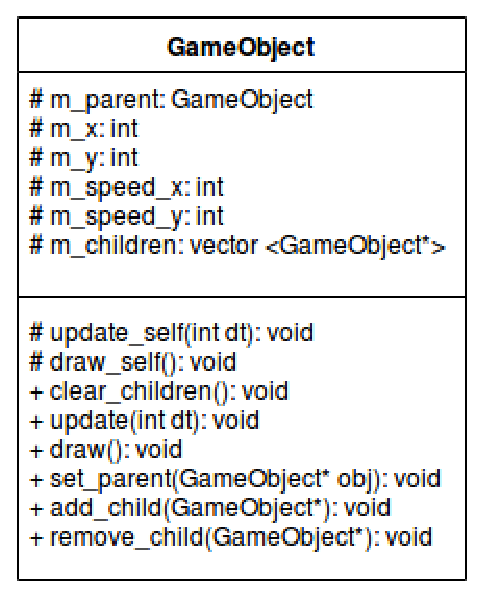
\includegraphics[keepaspectratio=true,scale=0.6]{figuras/game-object.eps}
      \caption[Modelagem inicial da classe \textit{GameObject}]
        {Modelagem inicial da classe \textit{GameObject}. Fonte: \textit{Autores}.}
      \label{game-object}
    \end{figure}

    Onde o método \textbf{\textit{update()}}, que é puramente virtual, trata de qualquer atualização do objeto a cada frame e o método \textbf{\textit{draw()}}, também puramente virtual, é responsável por renderizar o objeto na posição (\textit{x}, \textit{y}) a cada frame.

    É importante frisar que os métodos \textbf{\textit{update()}} e \textbf{\textit{draw()}} devem ser puramente virtuais, pois isso garante que qualquer classe que venha a extender de \textit{GameObject} seja obrigada a implementer suas próprias rotinas específicas de atualização e renderização.

    Além da classe \textit{GameObject}, os principais componentes da \textit{engine} a serem implementados são: módulo de vídeo, módulo de áudio, módulo de física e módulo de input.

    \subsubsection{Módulo de vídeo}

      O módulo de vídeo será responsável por renderizar qualquer tipo de imagem, animação e texto existente. Ele conterá as seguintes funcionalidades:

      \begin{itemize}
        \item Renderizar uma imagem de fundo;
        \item Renderizar uma \textit{sprite};
        \item Renderizar uma animação (como uma série de \textit{sprites});
        \item Movimentar horizontalmente uma imagem de fundo (\textit{horizontal scroll});
        \item Renderizar textos com uma determinada cor;
        \item Remover uma imagem, \textit{sprite}, texto ou animação que esteja renderizado da tela;
        \item Atualizar a renderização a cada frame, levando em consideração as posições \textit{x} e \textit{y} do \textit{sprite}, animação ou texto.
      \end{itemize}

      Deve-se lembrar que as imagens e textos que serão renderizados já estarão ajustados para a resolução e formato de cores corretos do GBA.

    \subsubsection{Módulo de áudio}

      O módulo de áudio ficará responsável por executar, no momento correto, qualquer música de fundo e efeito sonoro do jogo. Ele conterá as seguintes funcionalidades:

      \begin{itemize}
        \item Iniciar a execução de um efeito sonoro;
        \item Pausar a execução de um efeito sonoro;
        \item Parar a execução de um efeito sonoro;
        \item Iniciar a execução de uma música de fundo;
        \item Pausar a execução de uma música de fundo;
        \item Parar a execução de uma música de fundo.
      \end{itemize}

    \subsubsection{Módulo de física}

      O módulo de física terá como principal responsabilidade a detecção de colisões entre objetos do jogo. Ele conterá as seguintes funcionalidades:

      \begin{itemize}
        \item Simular, opcionalmente, a ação da gravidade em objetos do jogo;
        \item Detectar, opcionalmente, colisões entre objetos do jogo.
      \end{itemize}

    \subsubsection{Módulo de \textit{input}}

      O módulo de \textit{input} é responsável por receber qualquer pressionamento de qualquer um dos 10 botões e teclas do GBA.

  \subsection{Desenvolvimento do jogo}

    A implementação do jogo vai seguir o seguinte modelo de classes:

    \subsubsection{Objetos do jogo}

      O personagem principal, os itens coletáveis, plataformas, portais (para acesso e saída das fases) e elementos de HUD (\textit{heads-up display}) serão representados como \textit{game objects}.

      Abaixo se encontra a modelagem inicial dos objetos do jogo.

      \begin{figure}[H]
        \centering 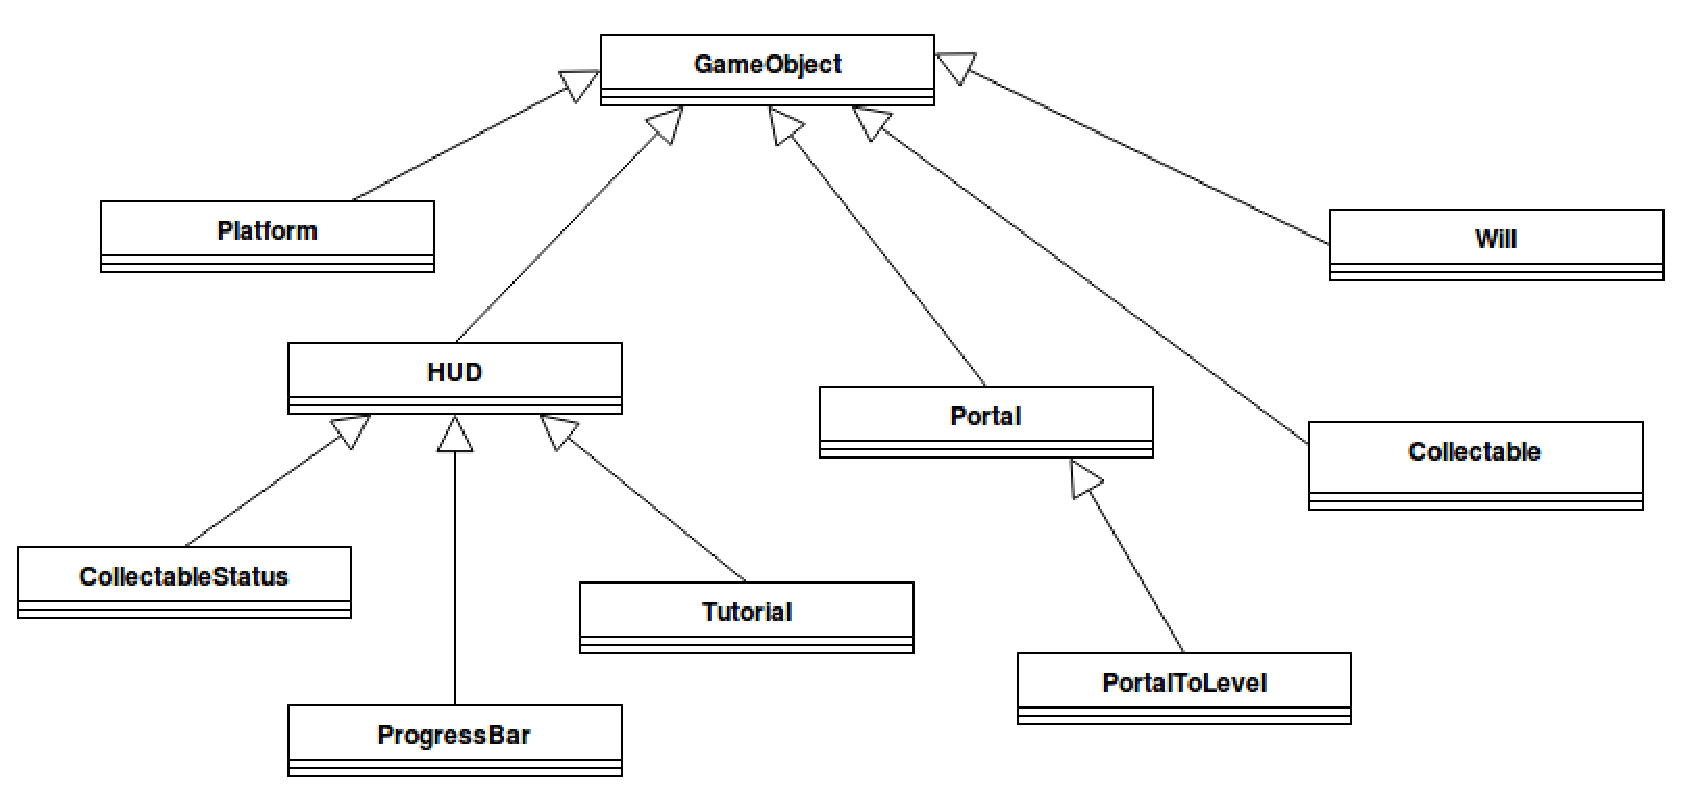
\includegraphics[keepaspectratio=true,scale=0.6]{figuras/class-diagram-1.eps}
        \caption[Modelagem inicial dos objetos do jogo]
          {Modelagem inicial dos objetos do jogo. Fonte: \textit{Autores}.}
        \label{game-object-children}
      \end{figure}

    \subsubsection{Níveis}

      A classe \textit{Level} contém a generalização de um nível no jogo. No jogo, os menus (principal e de seleção de fases), \textit{cutscenes}, fases e telas de vitória e derrota são representados como níveis do jogo.

      Abaixo se encontra a modelagem inicial dessas classes.

      \begin{figure}[H]
        \centering 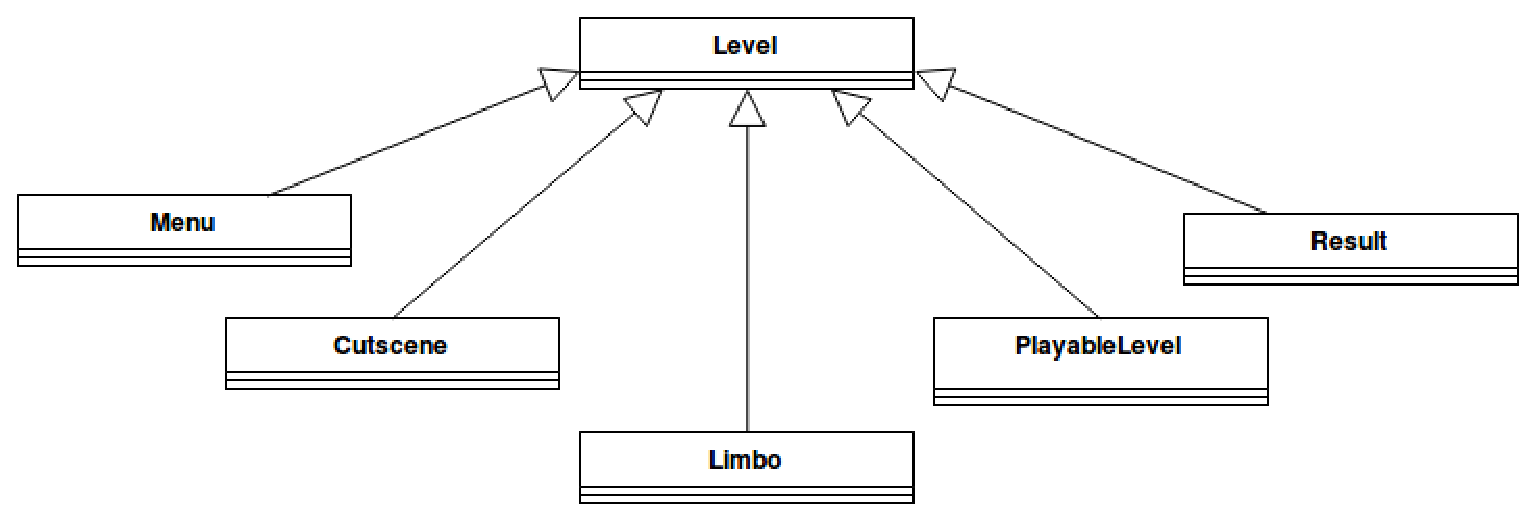
\includegraphics[keepaspectratio=true,scale=0.6]{figuras/class-diagram-2.eps}
        \caption[Modelagem inicial dos níveis do jogo]
          {Modelagem inicial dos níveis do jogo. Fonte: \textit{Autores}.}
        \label{game-object-levels}
      \end{figure}

    \subsubsection{Ajuste de recursos do jogo}

      Os recursos como imagens, áudios e arquivos de fonte do jogo precisarão ser editados para que possam ser carregados em memória e utilizados no GBA. No caso das imagens, por exemplo, serão modificadas características como dimensões e quantidade de cores a fim de diminuir seu tamanho para que possam ser convertidas para um formato utilizável no GBA.

% \section{Cronograma de desenvolvimento}

%   Abaixo se encontra o cronograma de desenvolvimento das tarefas planejadas para a conclusão do trabalho.

%   \begin{figure}[H]
%     \centering 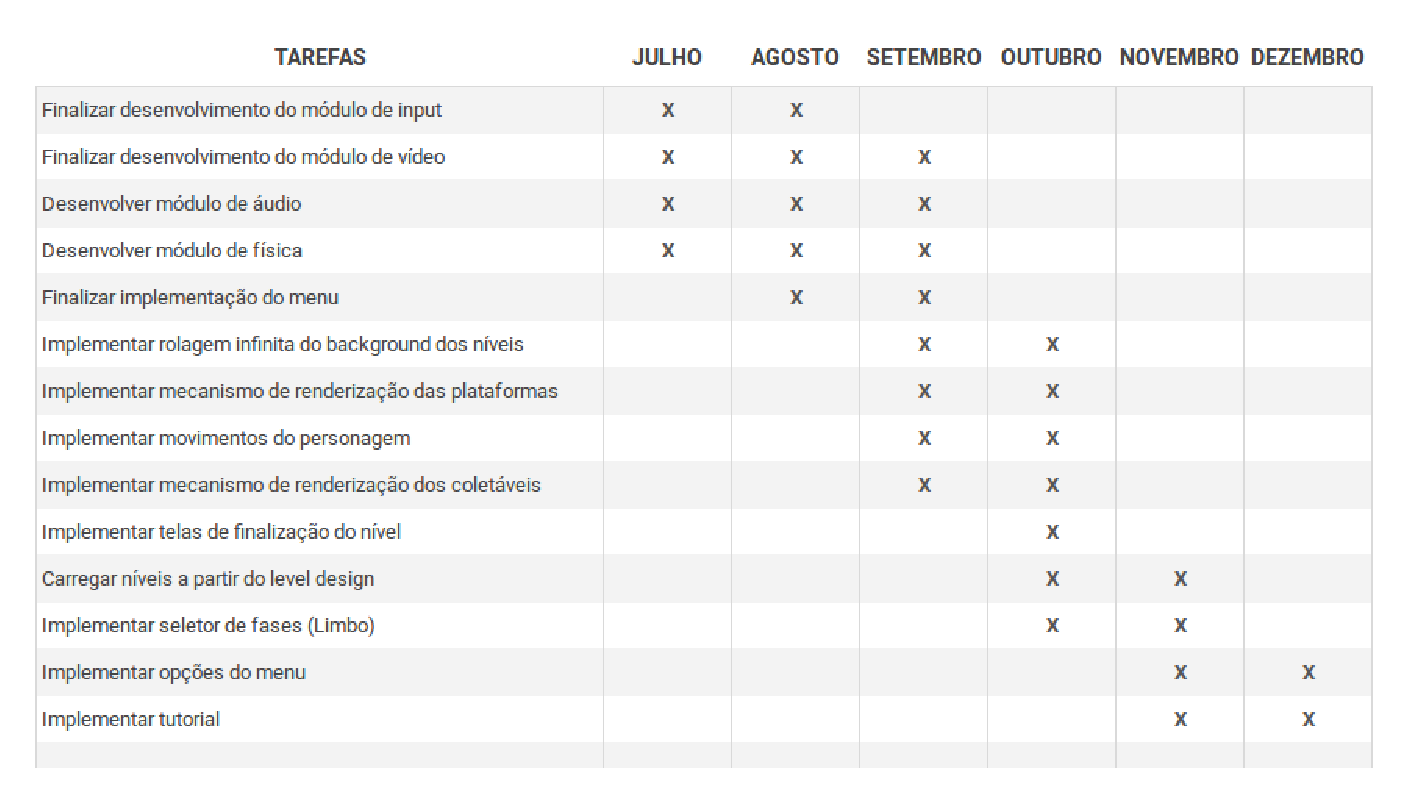
\includegraphics[keepaspectratio=true,scale=0.8]{figuras/cronograma.eps}
%     \caption[Cronograma de desenvolvimento]
%       {Cronograma de desenvolvimento. Fonte: \textit{Autores}.}
%     \label{cronograma}
%   \end{figure}
\chapter[Resultados Parciais]{Resultados Parciais}

\section{Protótipo inicial}

A fim de atestar a viabilidade do porte do jogo \textit{Traveling Will}, desenvolvido inicialmente para PC, para a plataforma \textit{Nintendo Game Boy Advance}, foi feita uma versão funcional do menu original do jogo, tendo essa versão sido testada em um GBA real. Para isso, a principal ferramenta utilizada foi a libtonc \cite{libtonc}, que nessa versão inicial fez o papel de engine do jogo.

Abaixo é possível comparar o menu principal do jogo original com o protótipo implementado sendo executado em um emulador de \textit{Game Boy Advance}:

\begin{figure}[H]
 \centering 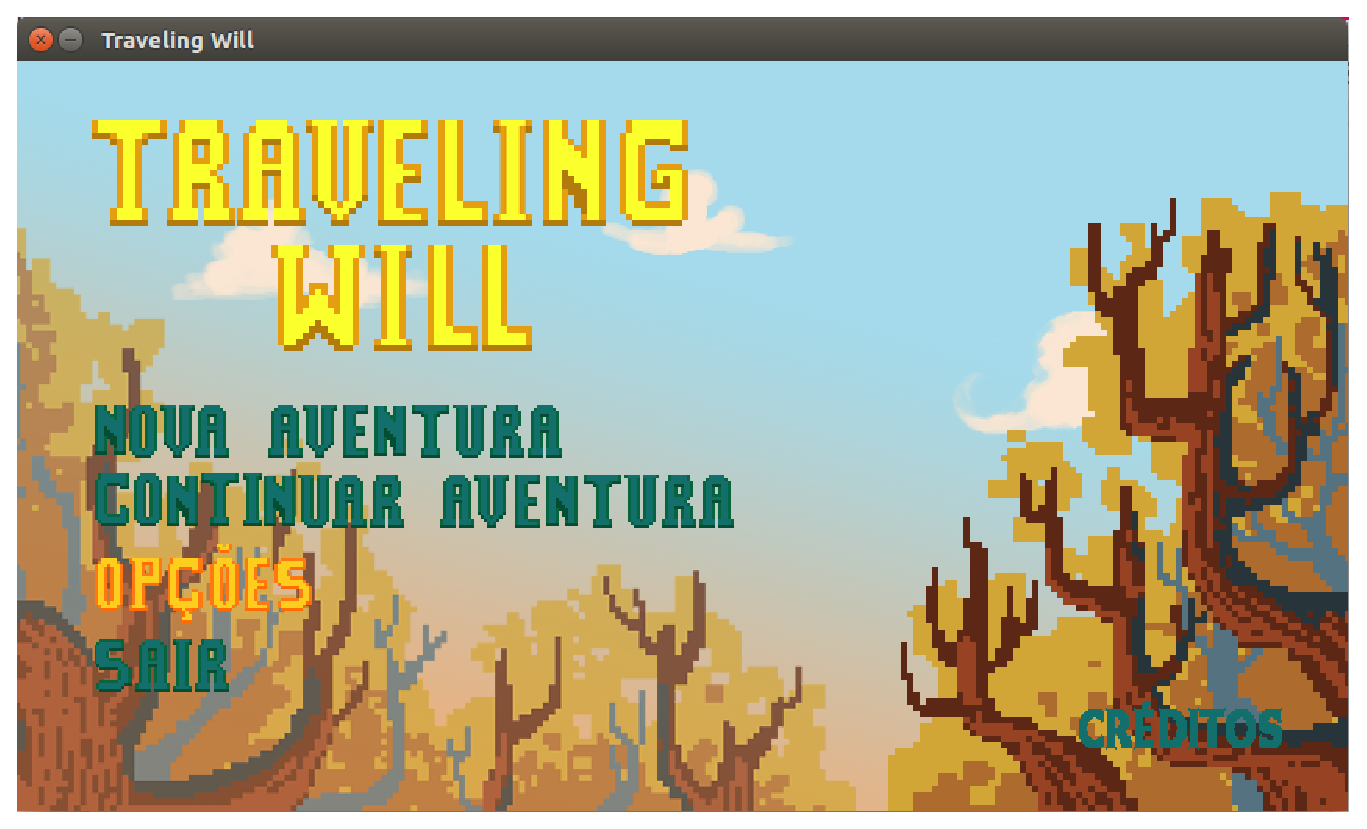
\includegraphics[keepaspectratio=true,scale=0.6]{figuras/tw-original-1.eps}
   \caption{Jogo original \textit{Traveling Will} sendo executado em um PC. Fonte: \textit{Autores}.}
   \label{tw-original-1}
\end{figure}

\begin{figure}[H]
 \centering 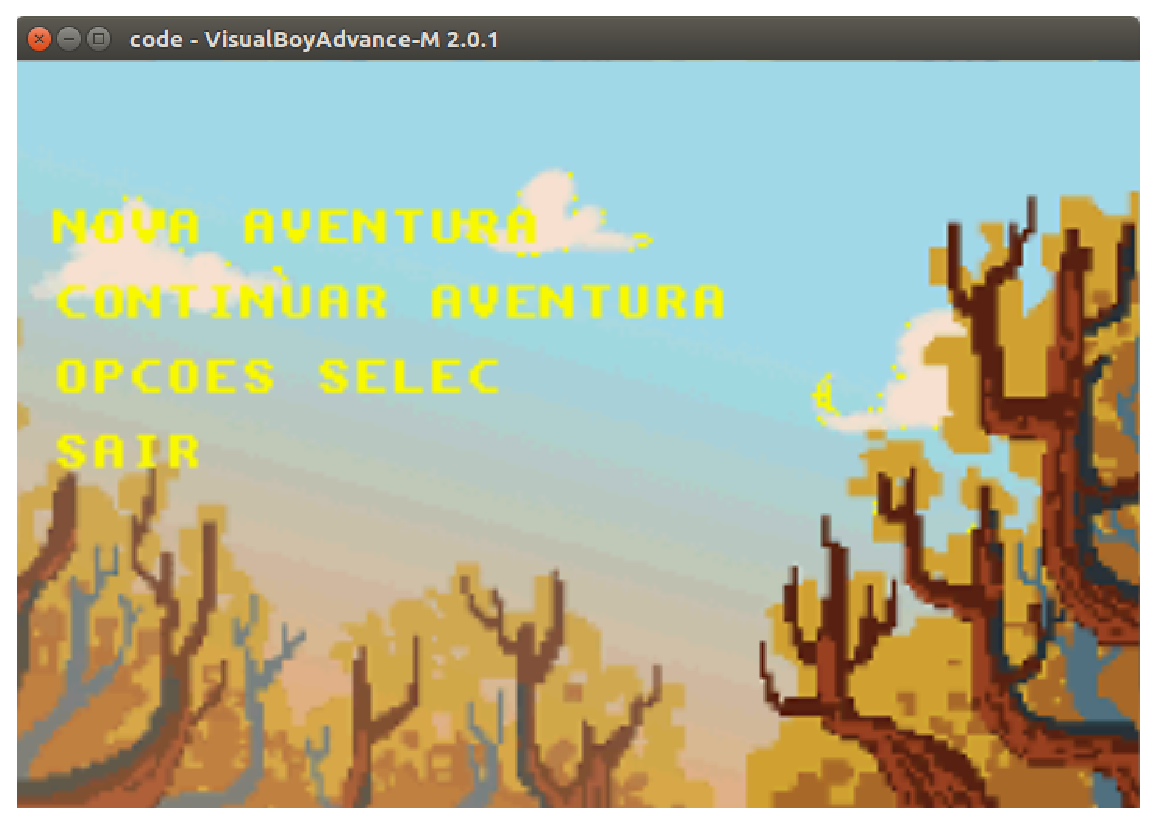
\includegraphics[keepaspectratio=true,scale=0.6]{figuras/tw-gba-1.eps}
   \caption{Protótipo implementado sendo executado em um emulador de GBA. Fonte: \textit{Autores}.}
   \label{tw-gba-1}
\end{figure}

\section{Desenvolvimento da \textit{engine}}

Após a finalização do protótipo inicial, foi iniciado o desenvolvimento da engine que irá substituir a libtonc na versão final do jogo. Ela irá padronizar a utilização dos recursos providos pelo GBA e irá conter um módulo de vídeo, áudio, \textit{input}, física, dentre outros.

Até o momento, o módulo de \textit{input} e parte do módulo de vídeo foram implementados.

\subsection{Módulo de \textit{input}}

Os estados dos botões do GBA ficam salvos em um registrador. Cada um desses estados é representado por um \textit{bit} no valor guardado por esse registrador. Sempre que um botão é apertado, o GBA automaticamente troca o valor guardado nesse registrador de tal forma que o \textit{bit} que representa o botão em questão passe a possuir valor 0. De forma similar, quando o botão é solto, o valor contido no \textit{bit} em questão é modificado para 1, seu valor padrão. Sendo assim, a checagem dos estados pode ser realizada facilmente utilizando \textit{bitmasks}. Por exemplo, caso se deseje checar um botão representado pelo \textit{bit} 2 (com a contagem começando em 0), basta pegar o resultado do \textit{AND} binário entre o valor guardado no registrador e a potência de 2 que possui como expotente o \textit{bit} em questão (4, nesse exemplo). Abaixo é possível vizualizar no código do módulo de input a definição das constantes que representam os botões, assim como a função utilizada para checar o estado de cada um deles:

\begin{minted}[frame=lines, linenos]
{c++}
#ifndef INPUT_H
#define INPUT_H

#include <stdbool.h>
#include "base_types.h"

#define BUTTON_A 1
#define BUTTON_B 2
#define BUTTON_SELECT 4
#define BUTTON_START 8
#define BUTTON_RIGHT 16
#define BUTTON_LEFT 32
#define BUTTON_UP 64
#define BUTTON_DOWN 128
#define BUTTON_R 256
#define BUTTON_L 512

#define N_BUTTON 10

int pressed_state[N_BUTTON];

void check_buttons_states();
bool pressed(int button);

#endif
\end{minted}
\makebox[\width]{Cabeçalho do módulo de input. Fonte: \textit{Autores}.}

\begin{minted}[frame=lines, linenos]
{c++}
#include "input.h"

volatile unsigned int *buttons_mem = (volatile unsigned int *)0x04000130;

void check_buttons_states() {
    for(int i = 0; i < N_BUTTON; i++) {
        pressed_state[i] = !((*buttons_mem) & (1 << i));
    }   
}

bool pressed(int button) {
    return pressed_state[button];
}
\end{minted}
\makebox[\width]{Código fonte do módulo de input. Fonte: \textit{Autores}.}

\subsection{Módulo de vídeo}

O módulo de vídeo deve possuir funções para controle do modo de vídeo, dos \textit{backgrounds} e da renderização das \textit{sprites}. Atualmente o módulo de vídeo desenvolvido trata apenas, de forma limitada, do modo de vídeo e do \textit{background}. Ele permite a renderização de um determinado \textit{background} desde que sejam passados a paleta de cores utilizada, um vetor com os \textit{tiles} utilizados no \textit{background} e um vetor representando o mapa de \textit{tiles} a ser utilizado para renderizar o \textit{background}. O módulo copia cada uma das informações passadas para as regiões de memória apropriadas. Atualmente, o módulo sempre utiliza o \textit{background} 2 e parte do princípio de que o modo utilizado não é baseado em \textit{bitmap}, não permitindo, portanto, o uso de múltiplos \textit{backgrounds}. Além disso, o módulo ainda não permite definir a posição exata de memória aonde o vetor de \textit{tiles} e o \textit{tilemap} deverão ser escritos, o que inviabiliza o uso de diferentes \textit{tilemaps}. Abaixo é possível visualizar a versão atual do código fonte do módulo de vídeo:

\begin{minted}[frame=lines, linenos]
{c++}
#include "video.h"

#include <string.h>

void reset_dispcnt() {
  REG_DISPCNT = 0;
}

void set_video_mode(int video_mode) {
  REG_DISPCNT |= video_mode;
}

void set_background_number(int background) {
  switch (background) {
    case 0:
      REG_DISPCNT |= 0x0100;
    case 1:
      REG_DISPCNT |= 0x0200;
    case 2:
      REG_DISPCNT |= 0x0400;
    case 3:
      REG_DISPCNT |= 0x0800;
  }
}

void set_background(const void *pal, int pal_len, const void *tiles, int tiles_len, const void *map, int map_len) {
  // Load palette
  memcpy(pal_bg_mem, pal, pal_len);
  // Load tiles into CBB 0
  memcpy(&tile_mem[0][0], tiles, tiles_len);
  // Load map into SBB 31
  memcpy(&se_mem[31][0], map, map_len);

  REG_BG2CNT = BG_CBB(0) | BG_SBB(31) | BG_8BPP | BG_REG_64x32;
}
\end{minted}
\makebox[\width]{Código fonte do módulo de vídeo. Fonte: \textit{Autores}.}

% \part{Aspectos Gerais}

\chapter[Aspectos Gerais]{Aspectos Gerais}

Estas instruções apresentam um conjunto mínimo de exigências necessárias a 
uniformidade de apresentação do relatório de Trabalho de Conclusão de Curso 
da FGA. Estilo, concisão e clareza ficam inteiramente sob a 
responsabilidade do(s) aluno(s) autor(es) do relatório.

As disciplinas de Trabalho de Conclusão de Curso (TCC) 01 e Trabalho de 
Conclusão de Curso (TCC) 02 se desenvolvem de acordo com Regulamento 
próprio aprovado pelo Colegiado da FGA. Os alunos matriculados nessas 
disciplinas devem estar plenamente cientes de tal Regulamento. 

\section{Composição e estrutura do trabalho}

A formatação do trabalho como um todo considera três elementos principais: 
(1) pré-textuais, (2) textuais e (3) pós-textuais. Cada um destes, pode se 
subdividir em outros elementos formando a estrutura global do trabalho, 
conforme abaixo (as entradas itálico são \textit{opcionais}; em itálico e
negrito são \textbf{\textit{essenciais}}):

\begin{description}
	\item [Pré-textuais] \

	\begin{itemize}
		\item Capa
		\item Folha de rosto
		\item \textit{Dedicatória}
		\item \textit{Agradecimentos}
		\item \textit{Epígrafe}
		\item Resumo
		\item Abstract
		\item Lista de figuras
		\item Lista de tabelas
		\item Lista de símbolos e
		\item Sumário
	\end{itemize}

	\item [Textuais] \

	\begin{itemize}
		\item \textbf{\textit{Introdução}}
		\item \textbf{\textit{Desenvolvimento}}
		\item \textbf{\textit{Conclusões}}
	\end{itemize}

	\item [Pós-Textuais] \
	
	\begin{itemize}
		\item Referências bibliográficas
		\item \textit{Bibliografia}
		\item Anexos
		\item Contracapa
	\end{itemize}
\end{description}

Os aspectos específicos da formatação de cada uma dessas três partes 
principais do relatório são tratados nos capítulos e seções seguintes.

No modelo \LaTeX, os arquivos correspondentes a estas estruturas que devem
ser editados manualmente estão na pasta \textbf{editáveis}. Os arquivos
da pasta \textbf{fixos} tratam os elementos que não necessitam de 
edição direta, e devem ser deixados como estão na grande maioria dos casos.

\section{Considerações sobre formatação básica do relatório}

A seguir são apresentadas as orientações básicas sobre a formatação do
documento. O modelo \LaTeX\ \textbf{já configura todas estas opções corretamente},
de modo que para os usuários deste modelo o texto de toda esta Seção é 
\textbf{meramente informativo}.

\subsection{Tipo de papel, fonte e margens}

Papel -- Na confecção do relatório deverá ser empregado papel branco no 
formato padrão A4 (21 cm x 29,7cm), com 75 a 90 g/m2.

Fonte -- Deve-se utilizar as fontes Arial ou Times New Roman no tamanho 12 
pra corpo do texto, com variações para tamanho 10 permitidas para a 
wpaginação, legendas e notas de rodapé. Em citações diretas de mais de três 
linhas utilizar a fonte tamanho 10, sem itálicos, negritos ou aspas. Os 
tipos itálicos são usados para nomes científicos e expressões estrangeiras, 
exceto expressões latinas.

Margens -- As margens delimitando a região na qual todo o texto deverá estar 
contido serão as seguintes: 

\begin{itemize}
	\item Esquerda: 03 cm;
	\item Direita	: 02 cm;
	\item Superior: 03 cm;
	\item Inferior: 02 cm. 
\end{itemize}

\subsection{Numeração de Páginas}

A contagem sequencial para a numeração de páginas começa a partir da 
primeira folha do trabalho que é a Folha de Rosto, contudo a numeração em 
si só deve ser iniciada a partir da primeira folha dos elementos textuais. 
Assim, as páginas dos elementos pré-textuais contam, mas não são numeradas 
e os números de página aparecem a partir da primeira folha dos elementos 
textuais, que se iniciam na Introdução. 

Os números devem estar em algarismos arábicos (fonte Times ou Arial 10) no 
canto superior direito da folha, a 02 cm da borda superior, sem traços, 
pontos ou parênteses. 

A paginação de Apêndices e Anexos deve ser contínua, dando seguimento ao 
texto principal.

\subsection{Espaços e alinhamento}

Para a monografia de TCC 01 e 02 o espaço entrelinhas do corpo do texto 
deve ser de 1,5 cm, exceto RESUMO, CITAÇÔES de mais de três linhas, NOTAS 
de rodapé, LEGENDAS e REFERÊNCIAS que devem possuir espaçamento simples. 
Ainda, ao se iniciar a primeira linha de cada novo parágrafo se deve 
tabular a distância de 1,25 cm da margem esquerda.

Quanto aos títulos das seções primárias da monografia, estes devem começar 
na parte superior da folha e separados do texto que o sucede, por um espaço 
de 1,5 cm entrelinhas, assim como os títulos das seções secundárias, 
terciárias. 

A formatação de alinhamento deve ser justificado, de modo que o texto fique 
alinhado uniformemente ao longo das margens esquerda e direita, exceto para 
CITAÇÕES de mais de três linhas que devem ser alinhadas a 04 cm da margem 
esquerda e REFERÊNCIAS que são alinhadas somente à margem esquerda do texto 
diferenciando cada referência.

\subsection{Quebra de Capítulos e Aproveitamento de Páginas}

Cada seção ou capítulo deverá começar numa nova pagina (recomenda-se que 
para texto muito longos o autor divida seu documento em mais de um arquivo 
eletrônico). 

Caso a última pagina de um capitulo tenha apenas um número reduzido de 
linhas (digamos 2 ou 3), verificar a possibilidade de modificar o texto 
(sem prejuízo do conteúdo e obedecendo as normas aqui colocadas) para 
evitar a ocorrência de uma página pouco aproveitada.

Ainda com respeito ao preenchimento das páginas, este deve ser otimizado, 
evitando-se espaços vazios desnecessários. 

Caso as dimensões de uma figura ou tabela impeçam que a mesma seja 
posicionada ao final de uma página, o deslocamento para a página seguinte 
não deve acarretar um vazio na pagina anterior. Para evitar tal ocorrência, 
deve-se reposicionar os blocos de texto para o preenchimento de vazios. 

Tabelas e figuras devem, sempre que possível, utilizar o espaço disponível 
da página evitando-se a \lq\lq quebra\rq\rq\ da figura ou tabela. 

\section{Cópias}

Nas versões do relatório para revisão da Banca Examinadora em TCC1 e TCC2, 
o aluno deve apresentar na Secretaria da FGA, uma cópia para cada membro da 
Banca Examinadora.

Após a aprovação em TCC2, o aluno deverá obrigatoriamente apresentar a 
versão final de seu trabalho à Secretaria da FGA na seguinte forma:

\begin{itemize}
	\item 01 cópia encadernada para arquivo na FGA;
	\item 01 cópia não encadernada (folhas avulsas) para arquivo na FGA;
	\item 01 cópia em CD de todos os arquivos empregados no trabalho.
\end{itemize}

A cópia em CD deve conter, além do texto, todos os arquivos dos quais se 
originaram os gráficos (excel, etc.) e figuras (jpg, bmp, gif, etc.) 
contidos no trabalho. Caso o trabalho tenha gerado códigos fontes e 
arquivos para aplicações especificas (programas em Fortran, C, Matlab, 
etc.) estes deverão também ser gravados em CD. 

O autor deverá certificar a não ocorrência de “vírus” no CD entregue a 
secretaria. 


% \chapter[Considerações finais]{Considerações finais}

Durante o desenvolvimento da \textit{engine} e do jogo, em diversos momentos bastante tempo foi empregado tentando entender detalhes da especificação do \textit{hardware} do GBA, como a definição da paleta de cores dos \textit{backgrounds} e \textit{sprites} serem bastante diferentes, o \textit{overlap} entre \textit{charblocks} e \textit{screenblocks} na região de memória VRAM, os diferentes canais de áudio que serviam para propósitos bem diferentes, a impossibilidade de se utilizar uma ferramenta de depuração de código, como \texttt{gdb}\footnote{\textit{GNU Debugger}, disponível em \url{https://bit.ly/2r2Wzza}}, entre outros. Esses impedimentos nos permitiram aprofundar nosso conhecimento em relação a como o \textit{hardware} do GBA funciona e como desenvolvedores de jogos para plataformas mais antigas resolviam problemas difíceis.

Por fim, como resultado final do trabalho, a pergunta de pesquisa pôde ser respondida afirmativamente, significando que foi possível portar o jogo \textit{Traveling Will}, desenvolvido originalmente para PC, para o \textit{Nintendo Gameboy Advance}, no contexto de um trabalho de conclusão de curso, com performance e jogabilidade próximos da versão para computador.

\section{Trabalhos futuros}

Como sugestões de trabalhos futuros, têm-se: melhoria do módulo de áudio para permitir carregar efeitos sonoros e pausar músicas durante a execução do jogo, implementação do carregamento e utilização de fontes no jogo, adição de elementos de HUD e seleção de fases, possibilidade de salvar o estado do jogo em memória e implementação de um desfragmentador de memória na classe \texttt{MemoryManager}.

\chapter[Trabalhos futuros]{Trabalhos futuros}

Como sugestões de trabalhos futuros, têm-se:

\begin{itemize}
  \item Melhoria do módulo de áudio;
  \item Possibilidade de salvar o estado do jogo em memória; e
  \item Implementação de um desfragmentador de memória na classe \texttt{MemoryManager}.
\end{itemize}
% \part{Texto e Pós Texto}

% \chapter[Elementos do Texto]{Elementos do Texto}

\section{Corpo do Texto}

O estilo de redação deve atentar a boa prática da linguagem técnica. Para a 
terminologia metrological usar o Vocabulário Internacional de Termos 
Fundamentais e Gerais de Metrologia \cite{inmetro2003}.

Grandezas dimensionais devem ser apresentadas em unidades consistentes com 
o Sistema Internacional de Unidades  (SI). Outras unidades podem ser usadas 
como unidades secundárias entre parenteses se necessário. Exceções são 
relacionadas a unidades não-SI usadas como identificadores comerciais como 
pro exemplo \lq\lq disquete de  3$\nicefrac{1}{2}$ polegadas\rq\rq. 

Na apresentação de números ao longo do texto usar virgula para separar a 
parte decimal de um número. Resultados experimentais devem ser apresentados 
com sua respectiva incerteza de medição.

\section{Títulos de capítulos e seções}

Recomendações de formatação de seções (texto informativo: o \LaTeX\
\textbf{já formata as seções automaticamente, se utilizado o comando
\texttt{\textbackslash section\{Nome da Seção\}}}):

\begin{description}

	\item \textbf{1 SEÇÃO PRIMÁRIA - MAIÚSCULAS; NEGRITO; TAMANHO 12;}

	\item 1.1 SEÇÃO SECUNDÁRIA – MAIÚSCULAS; NORMAL; TAMANHO 12; 

	\item \textbf{1.1.1 Seção terciária - Minúsculas, com exceção da 
	primeira letra; negrito; tamanho 12;}

	\item 1.1.1.1 Seção quaternária - Minúsculas, com exceção da primeira 
	letra; normal tamanho 12; 

 	\item \textit{1.1.1.1.1 Seção quinária - Minúsculas, com exceção da 
	primeira letra; itálico; tamanho 12.}

\end{description}

\section{Notas de rodapé}

Notas eventualmente necessárias devem ser numeradas de forma seqüencial ao 
longo do texto no formato 1, 2, 3... sendo posicionadas no rodapé de cada 
página na qual a nota é utilizada.\footnote{Como, por exemplo, esta nota. O \LaTeX\ tomará conta da numeração automaticamente.}

\section{Equações}

Equações matemáticas devem ser numeradas seqüencialmente e alinhadas a 
esquerda com recuo de 0,6 cm. Usar numerais arábicos entre parênteses, 
alinhado a direita, no formato Times New Roman de 9 pts. para numerara as 
equações como mostrado na Eq. \ref{eqn01} (novamente, o \LaTeX\ formata as
equações automaticamente).

Referências a equações no corpo do texto devem ser feitas como \lq\lq Eq. 
\ref{eqn01}\rq\rq\ quando no meio de uma frase ou como \lq\lq Equação 
\ref{eqn01}\rq\rq\ quando no inicio de uma sentença. Um espaçamento de 11 
pontos deve ser deixado acima, abaixo e entre equações subseqüentes. Para uma 
apresentação compacta das equações deve-se usar os símbolos e expressões 
matemáticos mais adequados e parênteses para evitar ambigüidades em 
denominadores. Os símbolos usados nas equações citados no texto devem 
apresentar exatamente a mesma formatação usada nas equações.
\begin{equation}
\label{eqn01}
	\frac{d\mathbf{C}}{dw} = \frac{du}{dw}\cdot \mathbf{F}_u + 
		\frac{dv}{dw}\cdot \mathbf{F}_v 
\end{equation}

O significado de todos os símbolos mostrados nas equações deve ser apresentado 
na lista de símbolos no inicio do trabalho, embora, em certas circunstancias o 
autor possa para maior clareza descrever o significado de certos símbolos no 
corpo do texto, logo após a equação.

Se uma equação aparecer no meio do parágrafo, como esta
\begin{equation}
x^n + y^n = z^n,
\end{equation}
onde $x, y, z, n \in \mathbf{N}$, o texto subsequente faz parte do parágrafo e 
não deve ser identado.

\section{Figuras e Gráficos}

As figuras devem ser centradas entre margens e identificadas por uma legenda 
alinhada a esquerda com recuo especial de deslocamento de 1,8 cm, com mostrado 
na Fig. (\ref{fig01}). O tamanho das fontes empregadas nos rótulos e anotações 
usadas nas figuras deve ser compatível com o usado no corpo do texto. Rótulos e 
anotações devem estar em português, com todas as grandezas mostradas em 
unidades do SI (Sistema Internacional de unidades) (mais uma vez, o \LaTeX\
cuidará dos aspectos de formatação e fonte das figuras).

Todas as figuras, gráficos e fotografias devem ser numeradas e referidas no 
corpo do texto adotando uma numeração seqüencial de identificação. As figuras e 
gráficos devem ser claras e com qualidade adequada para eventual reprodução 
posterior tanto em cores quanto em preto-e-branco.

As abscissas e ordenadas de todos os gráficos devem ser rotuladas com seus 
respectivos títulos em português seguida da unidade no SI que caracteriza a 
grandes entre colchetes. 

A referência explícita no texto à uma figura deve ser feita como 
\lq\lq Fig. \ref{fig01}\rq\rq\ quando no meio de uma frase ou como 
\lq\lq Figura \ref{fig01}\rq\rq\ quando no início da mesma. Referencias 
implícitas a uma dada figura devem ser feitas entre parênteses como 
(Fig. \ref{fig01}). Para referências a mais de uma figura as mesmas regras 
devem ser aplicadas usando-se o plural adequadamente. Exemplos:

\begin{itemize}
	\item \lq\lq Após os ensaios experimentais, foram obtidos os resultados 
	mostrados na Fig. \ref{fig01}, que ...\rq\rq
	\item \lq\lq A Figura \ref{fig01} apresenta os resultados obtidos, onde 
	pode-se observar que ...\rq\rq
	\item \lq\lq As Figuras 1 a 3 apresentam os resultados obtidos, 
	...\rq\rq
	\item \lq\lq Verificou-se uma forte dependência entre as variáveis citadas 
	(Fig. \ref{fig01}), comprovando ...\rq\rq
\end{itemize}

Cada figura deve ser posicionada o mais próxima possível da primeira citação 
feita à mesma no texto, imediatamente após o parágrafo no qual é feita tal 
citação, se possível, na mesma página. Em \LaTeX\, o comando \texttt{\textbackslash label} deve suceder o comando \texttt{\textbackslash caption} para que as referências às figuras fiquem com a numeração correta.
\begin{figure}[h]
	\centering
	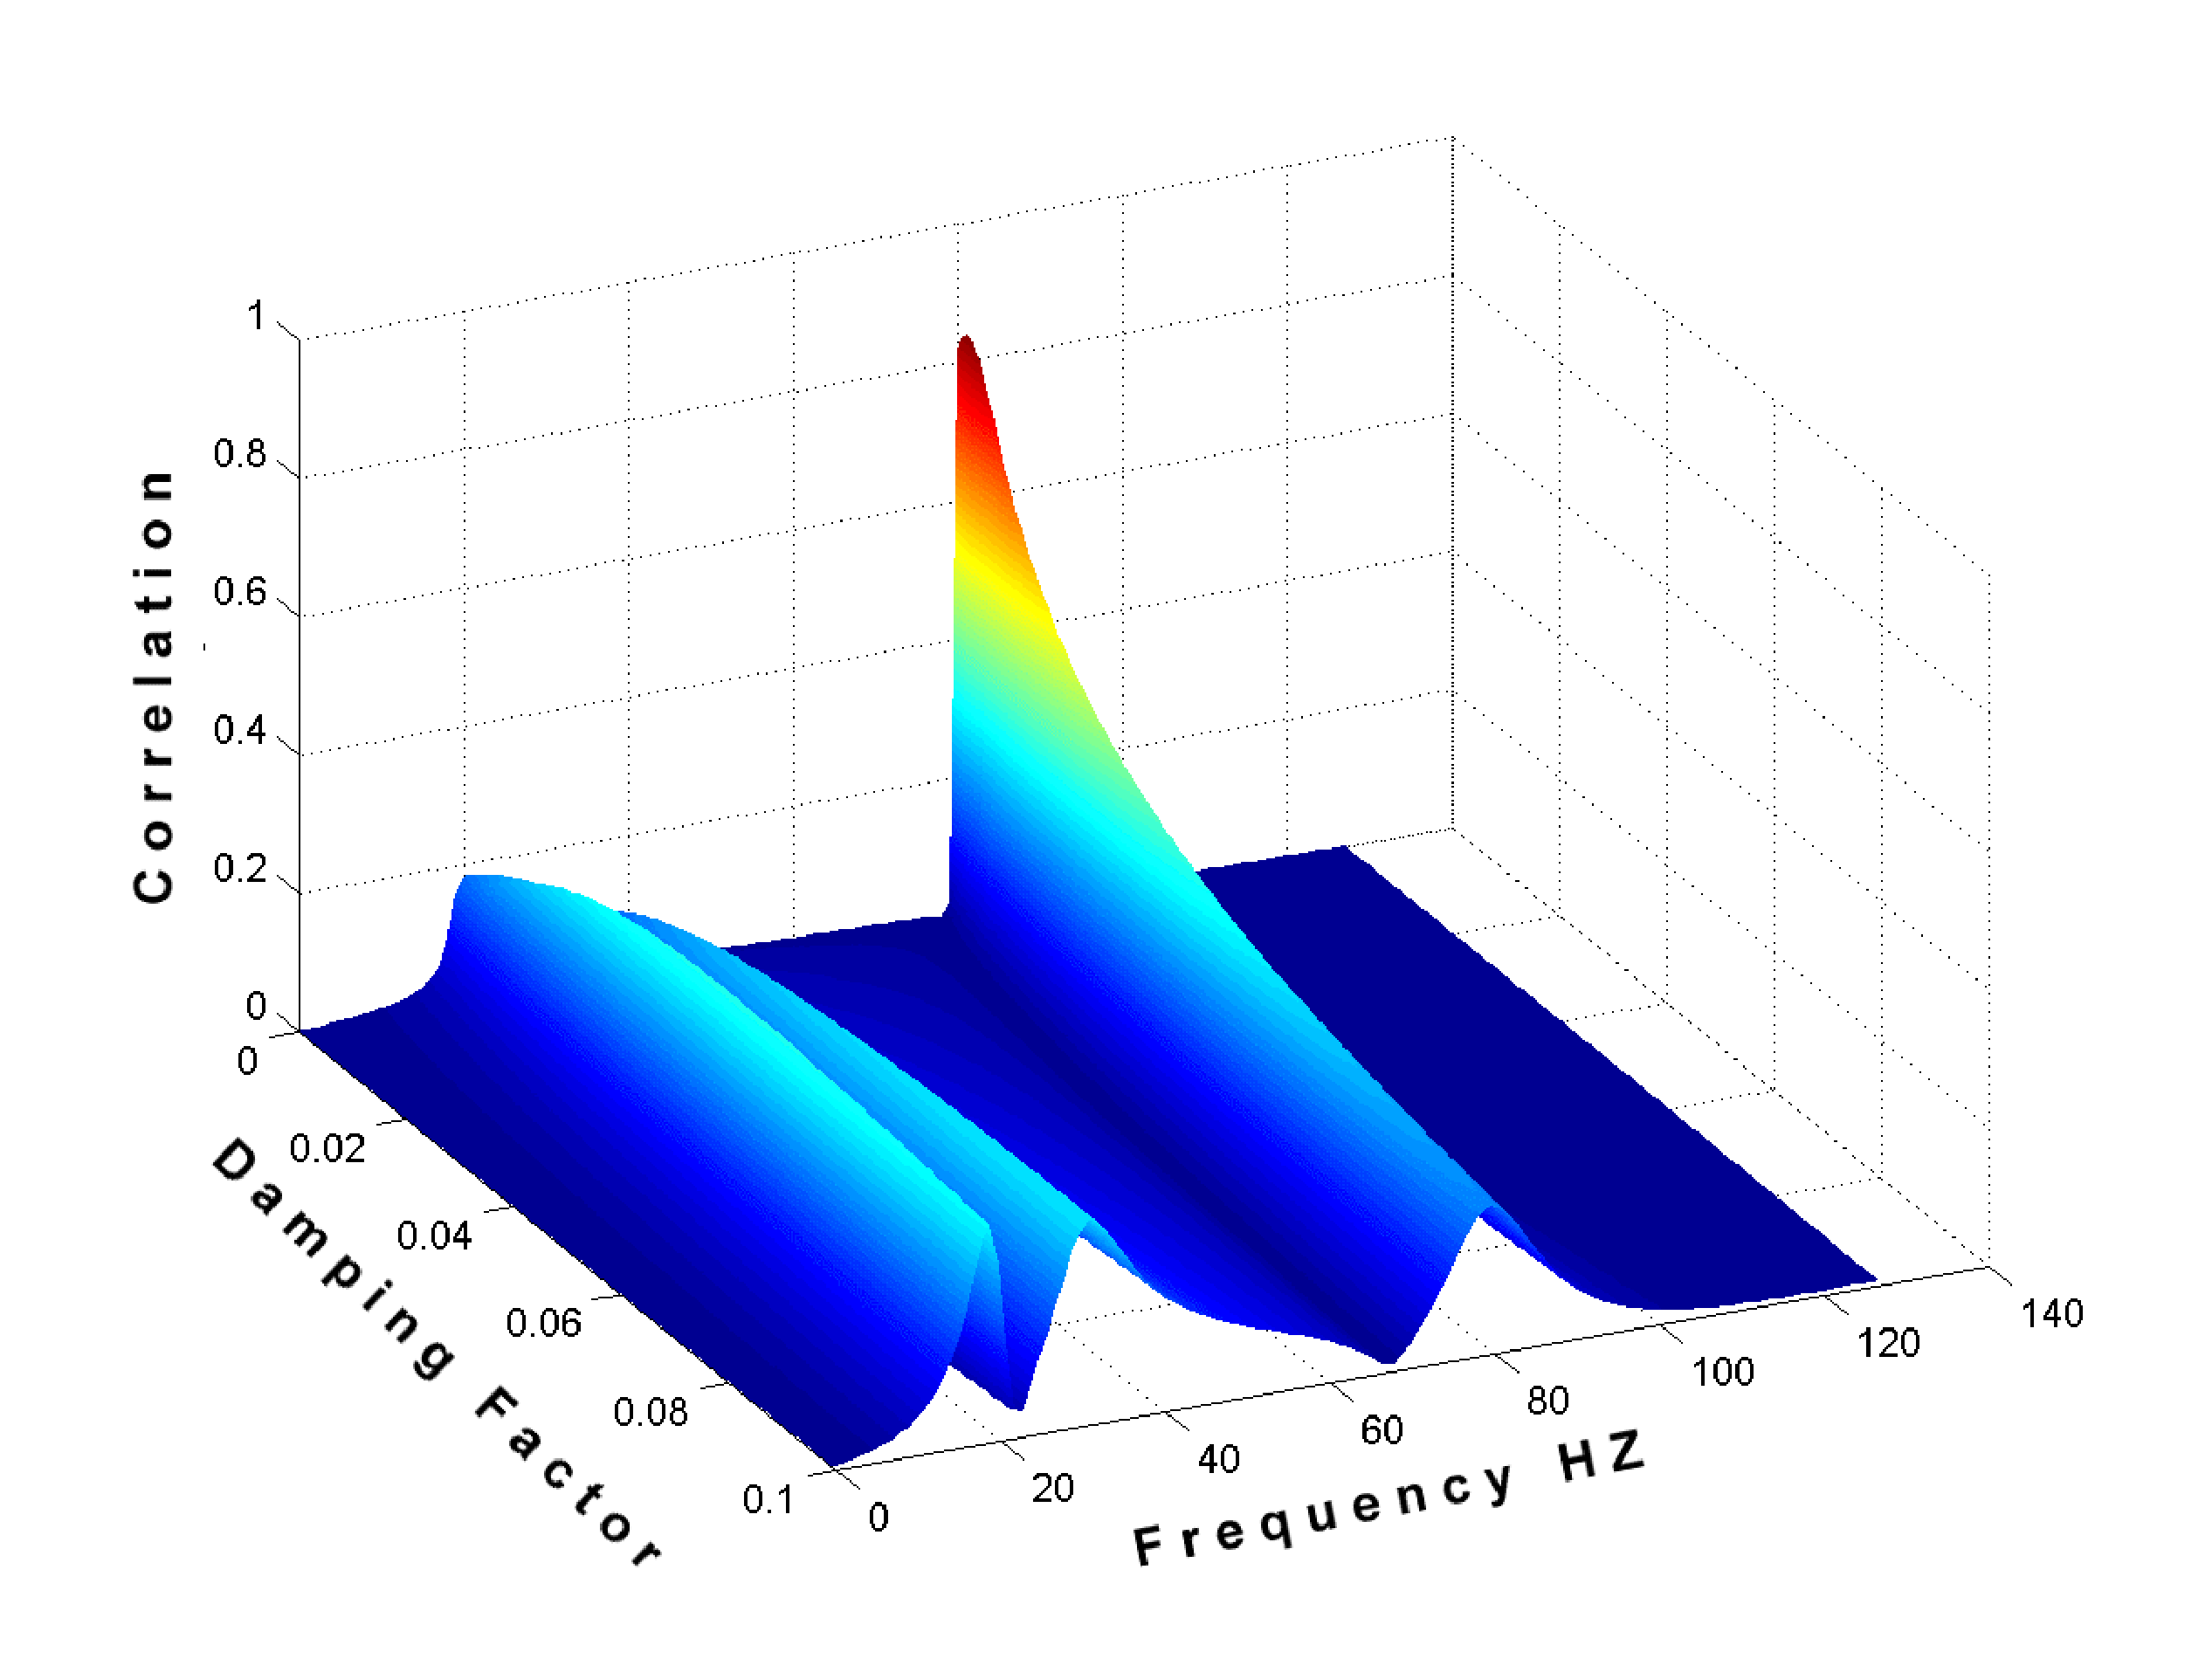
\includegraphics[keepaspectratio=true,scale=0.3]{figuras/fig01.eps}
	\caption{Wavelets correlation coefficients}
	\label{fig01}
\end{figure}

\section{Tabela}

As tabelas devem estar centradas entre margens e identificadas por uma legenda 
alinhada a esquerda, com recuo especial de deslocamento de 1,8 cm, posicionada 
acima da tabela com mostrado na Tab. \ref{tab01}, a título de 
exemplo. O tamanho das fontes empregadas nos rótulos e anotações usadas nas 
tabelas deve ser compatível com o usado no corpo do texto. Rótulos e anotações 
devem estar em português. Um espaçamento de 11 pts deve ser deixado entre a 
legenda e a tabela, bem como após a tabela. A numeração, a fonte e a formatação
são automáticas quando se usa o \LaTeX.

As grandezas dimensionais mostradas em cada tabela devem apresentar unidades 
consistentes com o SI. As unidades de cada variável devem ser mostradas apenas 
na primeira linha e/ou coluna da tabela, entre colchetes 

A referência explícita no texto à uma dada tabela deve ser feita como 
\lq\lq Tab. \ref{tab01}\rq\rq\ quando no meio de uma frase ou como 
\lq\lq Tabela \ref{tab01}\rq\rq\ quando no início da mesma. Referências 
implícitas a uma dada tabela devem ser feitas entre parênteses como 
(Tab. \ref{tab01}). Para referências a mais de uma tabela as mesmas 
regras devem ser aplicadas usando-se o plural adequadamente. Exemplos:
\begin{itemize}
	\item \lq\lq Após os ensaios experimentais, foram obtidos os resultados 
	mostrados na Tab. \ref{tab01}, que ...\rq\rq
	\item \lq\lq A Tabela \ref{tab01} apresenta os resultados obtidos, onde 
	pode-se observar que ...\rq\rq
	\item \lq\lq As Tabelas 1 a 3 apresentam os resultados obtidos, ...\rq\rq
	\item \lq\lq Verificou-se uma forte dependência entre as variáveis citadas 
	(Tab. \ref{tab01}), comprovando ...\rq\rq
\end{itemize}

Cada tabela deve ser posicionada o mais próxima possível da primeira citação 
feita à mesma no texto, imediatamente após o parágrafo no qual é feita a 
citação, se possível, na mesma página.

\begin{table}[h]
	\centering
	\caption{Propriedades obtidades após processamento}
	\label{tab01}
	
	\begin{tabular}{ccc}
		\toprule
		\textbf{Processing type} & \textbf{Property 1} (\%) & 
		\textbf{Property 2} $[\mu m]$ \\
		\midrule
		Process 1 & 40.0 & 22.7 \\
		Process 2 & 48.4 & 13.9 \\
		Process 3 & 39.0 & 22.5 \\
		Process 4 & 45.3 & 28.5 \\
		\bottomrule
	\end{tabular}
\end{table}

\section{Citação de Referências}

Referencias a outros trabalhos tais como artigos, teses, relatórios, etc. devem 
ser feitas no corpo do texto devem estar de acordo com a norma corrente ABNT 
NBR 6023:2002 (ABNT, 2000), esta ultima baseada nas normas ISO 690:1987:
\begin{itemize}
	\item \lq\lq \citeonline{bordalo1989}, mostraram que...\rq\rq

	\item \lq\lq Resultados disponíveis em \cite{coimbra1978}, \cite{clark1986} 
	e \cite{sparrow1980}, mostram que...\rq\rq
\end{itemize}

Para referências a trabalhos com até dois autores, deve-se citar o nome de 
ambos os autores, por exemplo: \lq\lq \citeonline{soviero1997}, mostraram 
que...\rq\rq


% \chapter[Elementos do Pós-Texto]{Elementos do Pós-Texto}

Este capitulo apresenta instruções gerais sobre a elaboração e formatação dos 
elementos do pós-texto a serem apresentados em relatórios de Projeto de 
Graduação. São abordados aspectos relacionados a redação de referências 
bibliográficas, bibliografia, anexos e contra-capa.

\section{Referências Bibliográficas}

O primeiro elemento do pós-texto, inserido numa nova página, logo após o último 
capítulo do trabalho, consiste da lista das referencias bibliográficas citadas 
ao longo do texto.

Cada referência na lista deve ser justificada entre margens e redigida no 
formato Times New Roman com 11pts. Não é necessário introduzir uma linha em 
branco entre referências sucessivas.

A primeira linha de cada referencia deve ser alinhada a esquerda, com as demais 
linhas da referencia deslocadas de 0,5 cm a partir da margem esquerda. 

Todas as referências aparecendo na lista da seção \lq\lq Referências 
Bibliográficas\rq\rq\ devem estar citadas no texto. Da mesma forma o autor deve 
verificar que não há no corpo do texto citação a referências que por 
esquecimento não forma incluídas nesta seção.

As referências devem ser listadas em ordem alfabética, de acordo com o último 
nome do primeiro autor. Alguns exemplos de listagem de referencias são 
apresentados no Anexo I.

Artigos que ainda não tenham sido publicados, mesmo que tenham sido submetidos 
para publicação, não deverão ser citados. Artigos ainda não publicados mas que 
já tenham sido aceitos para publicação devem ser citados como \lq\lq in 
press\rq\rq.

A norma \cite{NBR6034:2000}, que regulamenta toda a formatação a ser usada na 
elaboração de referências a diferente tipos de fontes de consulta, deve ser 
rigidamente observada. Sugere-se a consulta do trabalho realizado por 
\cite{arruda2007}, disponível na internet.

\section{Anexos}

As informações citadas ao longo do texto como \lq\lq Anexos\rq\rq\ devem ser 
apresentadas numa seção isolada ao término do trabalho, após a seção de 
referências bibliográficas. Os anexos devem ser numerados seqüencialmente em 
algarismos romanos maiúsculos (I, II, III, ...). A primeira página dos anexos 
deve apresentar um índice conforme modelo apresentado no Anexo I, descrevendo 
cada anexo e a página inicial do mesmo.

A referência explícita no texto à um dado anexo deve ser feita como 
\lq\lq Anexo 1\rq\rq. Referências implícitas a um dado anexo devem ser feitas 
entre parênteses como (Anexo I). Para referências a mais de um anexo as mesmas 
regras devem ser aplicadas usando-se o plural adequadamente. Exemplos:
\begin{itemize}
	\item \lq\lq Os resultados detalhados dos ensaios experimentais são 
	apresentados no Anexo IV, onde ...\rq\rq

	\item \lq\lq O Anexo I apresenta os resultados obtidos, onde pode-se 
	observar que ...\rq\rq

	\item \lq\lq Os Anexos I a IV apresentam os resultados obtidos ...\rq\rq

	\item \lq\lq Verificou-se uma forte dependência entre as variáveis citadas 
	(Anexo V), comprovando ...\rq\rq
\end{itemize}



\bookmarksetup{startatroot}

\postextual

\bibliography{bibliografia}
% \begin{apendicesenv}

\partapendices

\chapter{Primeiro Apêndice}

Texto do primeiro apêndice.

\chapter{Segundo Apêndice}

Texto do segundo apêndice.

\end{apendicesenv}

% \begin{anexosenv}

\partanexos

\chapter{Primeiro Anexo}

Texto do primeiro anexo.

\chapter{Segundo Anexo}

Texto do segundo anexo.

\end{anexosenv}


\printindex

\end{document}

